\documentclass[10pt]{article}
\usepackage[utf8]{inputenc}
\usepackage{pgfplots}
\pgfplotsset{compat=1.15}
\usepackage{mathrsfs}
\usetikzlibrary{arrows}
\pagestyle{empty}
\begin{document}
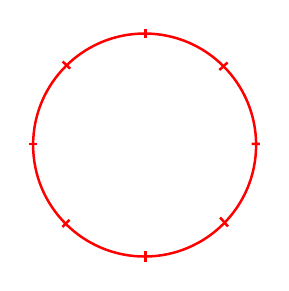
\begin{tikzpicture}[x=1.0cm,y=1.0cm]
%\begin{axis}[x=1.0cm,y=1.0cm,axis lines=middle,ymajorgrids=true,xmajorgrids=true, xmin=0,xmax=3,ymin=0,ymax=3,xtick={0,1,...,3},ytick={0,1,...,3}]
%\clip(0,0) rectangle (3,3);
\draw [line width=0.9pt,color=red] (1.4692446893009805,1.485473559484133) circle (1.4160262922671587cm);
\draw [line width=0.9pt,color=red] (0.4256901612340227,0.4437574268792198)-- (0.5158378930922598,0.5339051587374565);
\draw [line width=0.9pt,color=red] (1.48,0.)-- (1.48,0.14233852398668978);
\draw [line width=0.9pt,color=red] (2.4282370447769273,0.5647927937021489)-- (2.52787401156761,0.45092197451279714);
\draw [line width=0.9pt,color=red] (2.829093469411946,1.500739986657983)-- (2.931963988531224,1.4990807847367043);
\draw [line width=0.9pt,color=red] (2.418537761142508,2.438078648458227)-- (2.522919345399414,2.5329709977826864);
\draw [line width=0.9pt,color=red] (0.1,1.5)-- (0.,1.5);
\draw [line width=0.9pt,color=red] (0.4289919362229539,2.545712998873254)-- (0.5238842855474137,2.455565267015017);
\draw [line width=0.9pt,color=red] (1.48,2.84)-- (1.48,2.96);
\begin{scriptsize}
%\draw[color=red] (0.778527091560426,2.607288645837755) node {$c$};
%\draw[color=red] (0.5690574279869282,0.46925345901863996) node {$f$};
%\draw[color=red] (1.6164057458544174,0.13699123403999378) node {$g$};
%\draw[color=red] (2.4109458490642375,0.49814582640808747) node {$h$};
%\draw[color=red] (2.894893002837491,1.4515939502598547) node {$i$};
%\draw[color=red] (2.569853869706201,2.4628268088905174) node {$j$};
%\draw[color=red] (0.07066409051895045,1.6827328893754347) node {$k$};
%\draw[color=red] (0.4173724991923262,2.484496084432603) node {$l$};
%\draw[color=red] (1.6164057458544174,2.9684432382058485) node {$m$};
\end{scriptsize}
%\end{axis}
\end{tikzpicture}
\end{document} 